%!TEX root = ../dissertation.tex

\chapter{Methodology}
\label{chp:methodology}
This chapter outlines the methodology employed in the development and implementation of the Social Media Kit (SMKIT) project. It provides a comprehensive explanation of the tools, techniques, and processes used to design, build, and implement the system. The chapter begins with an overview of the system architecture, followed by detailed discussions on data collection, processing, and the integration of various components.
This chapter sets the foundation for understanding the practical implementation of SMKIT, which will be further detailed in the subsequent chapters.


\section{Introduction}
\label{sec:introduction}
This section introduces the methodology used for developing the Social Media Kit (SMKIT). It provides an overview of the key techniques and tools employed throughout the development process, providing the foundation for the work presented in this thesis. The methodology chapter serves as a detailed explanation of how the objectives of SMKIT were achieved, with a focus on the following key areas:

\begin{itemize}
    \item \textbf{System Design and Architecture}: A comprehensive description of the system architecture of SMKIT, including the design decisions made to ensure the system’s scalability and functionality.
    \item \textbf{Data Collection and Preparation}: An overview of the data extraction techniques used, including web scraping tools and methods for cleaning and transforming the data into usable formats.
    \item \textbf{Implementation Process}: A detailed explanation of the implementation phase, where the system was developed and integrated with components like Negapedia and social media platforms.
    \item \textbf{Challenges and Limitations}: A reflection on the obstacles faced during the project and the limitations of the system that are important to consider when interpreting the results.
\end{itemize}

Each of these areas will be explored in detail in the subsequent sections of this chapter. By providing a comprehensive explanation of the methodologies used, this chapter ensures that the development process of SMKIT is well-understood.

The following sections will build upon this introductory overview, examining each of the mentioned aspects in greater detail to provide a complete picture of the technical and conceptual approaches adopted in the development of SMKIT.


\section{System Design and Architecture}
\label{sec:system_design_architecture}
This section explains the design decisions made for the Social Media Kit (SMKIT), including the overall system architecture, the key components that make up the system, and how these components interact to achieve the desired functionality. The system is designed to automate the generation and sharing of content on social media platforms, leveraging data from websites that integrate Open Graph (OG) tags or from the Negapedia website through a dedicated module for contextual analysis and content creation.

The architecture of SMKIT is based on a modular and scalable approach, allowing for flexibility in future development. Below are the key aspects of the system design:

\begin{itemize}
    \item \textbf{Modular Architecture}: The system is built using a modular architecture, where each component or unit has a specific responsibility. This allows for easy maintenance and the potential for future upgrades. \begin{comment} The key components include:
    \begin{itemize}
        \item \textbf{Data Extraction Component}: Responsible for extracting data from external sources, such as websites with Open Graph (OG) tags or Negapedia specific data through web scraping.
        \item \textbf{Data Transformation Component}: Handles data cleaning, transformation, and analysis, converting raw data into structured and usable formats.
        \item \textbf{Content Creation Component}: Uses the processed data to automatically generate content for social media posts, including text and multimedia.
        \item \textbf{Social Media Posting Component}: Manages the process of posting content, previously extracted into structured and usable formats, to various social media platforms (e.g., Twitter, Facebook) through the use of APIs.
    \end{itemize} \end{comment}
    
    
    \item \textbf{Scalability}: SMKIT is designed with scalability in mind. The system can handle multiple social media platforms and expand to include additional sources of data and content generation features. By using a modular structure, new components can be added without disrupting existing functionality.
    
    \item \textbf{Data Flow}: The data flow in SMKIT is sequential and structured. The process begins with the extraction of data from external sources, followed by cleaning and transformation, content generation, and finally, posting to social media platforms. \begin{comment} The following diagram illustrates the flow of data through the system:
    
    \begin{figure}[ht]
        \centering
        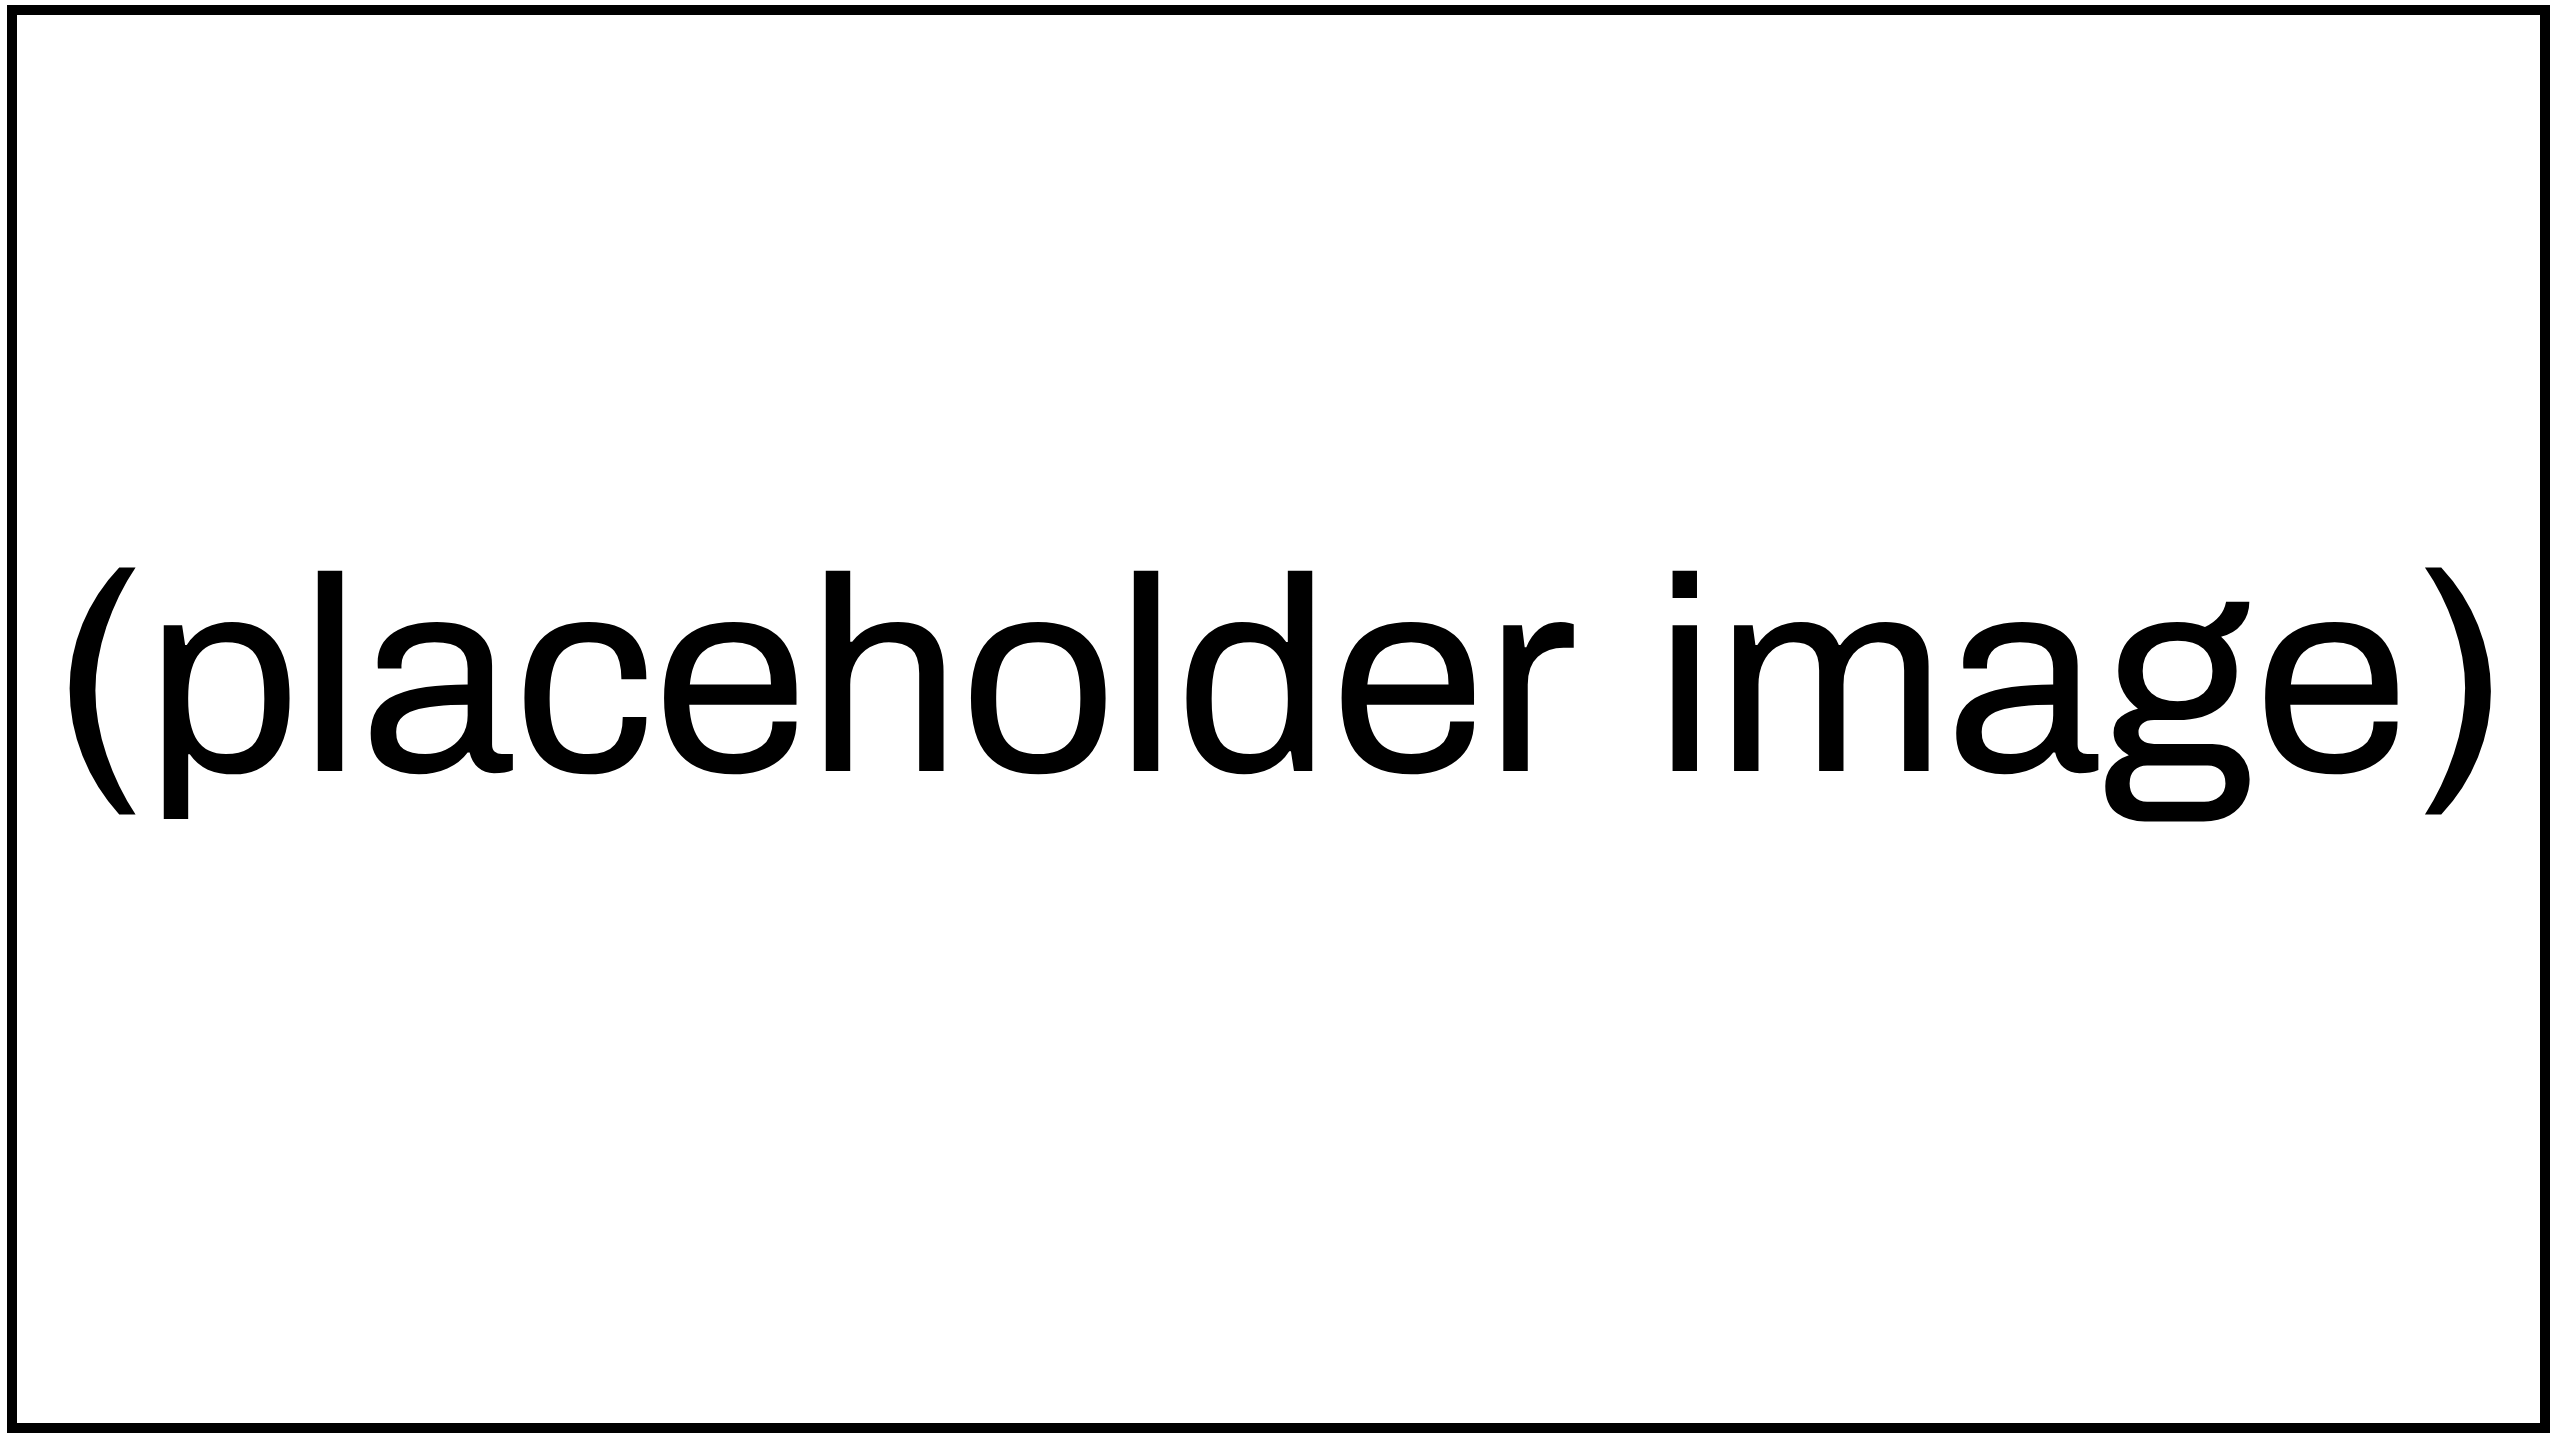
\includegraphics[width=0.8\textwidth]{figures/methodology/placeholder_image.png}
        \caption{System Architecture and Data Flow}
        \label{fig:system_architecture}
    \end{figure} \end{comment}

\end{itemize}

\subsection{System Architecture Overview}
\label{subsec:system_architecture_overview}
The system architecture of the Social Media Kit (SMKIT) is designed with a modular approach to ensure scalability, flexibility, and ease of maintenance. The architecture integrates several key components that work together to automate the extraction, processing, generation, and sharing of content on social media platforms. Below is an overview of how these components interact:

\begin{itemize}
    \item \textbf{Data Extraction Component}: The system begins by extracting raw data from external sources. This data extraction process can be achieved through web scraping, which provide the foundational content for further processing.

    \item \textbf{Data Transformation Component}: Once the raw data is collected, it is passed on to the data transformation component. This component is responsible for cleaning, structuring, and transforming the raw data into a usable format. It processes unstructured text to extract key insights, removes irrelevant or noisy data, and organizes the content into predefined formats.
    
    \item \textbf{Social Media Posting Component}: Finally, the transformed content is sent to the social media posting component. This component manages the process of sharing the content across various platforms like Twitter and Facebook, utilizing platform-specific APIs to ensure seamless posting.
\end{itemize}

The modularity of the architecture allows for flexibility in extending the system to include new data sources with eventually new tailored predefined formats, additional social media platforms, or advanced content generation techniques, such as sentiment analysis and machine learning-based content optimization.

\begin{comment}
\begin{figure}[ht]
    \centering
    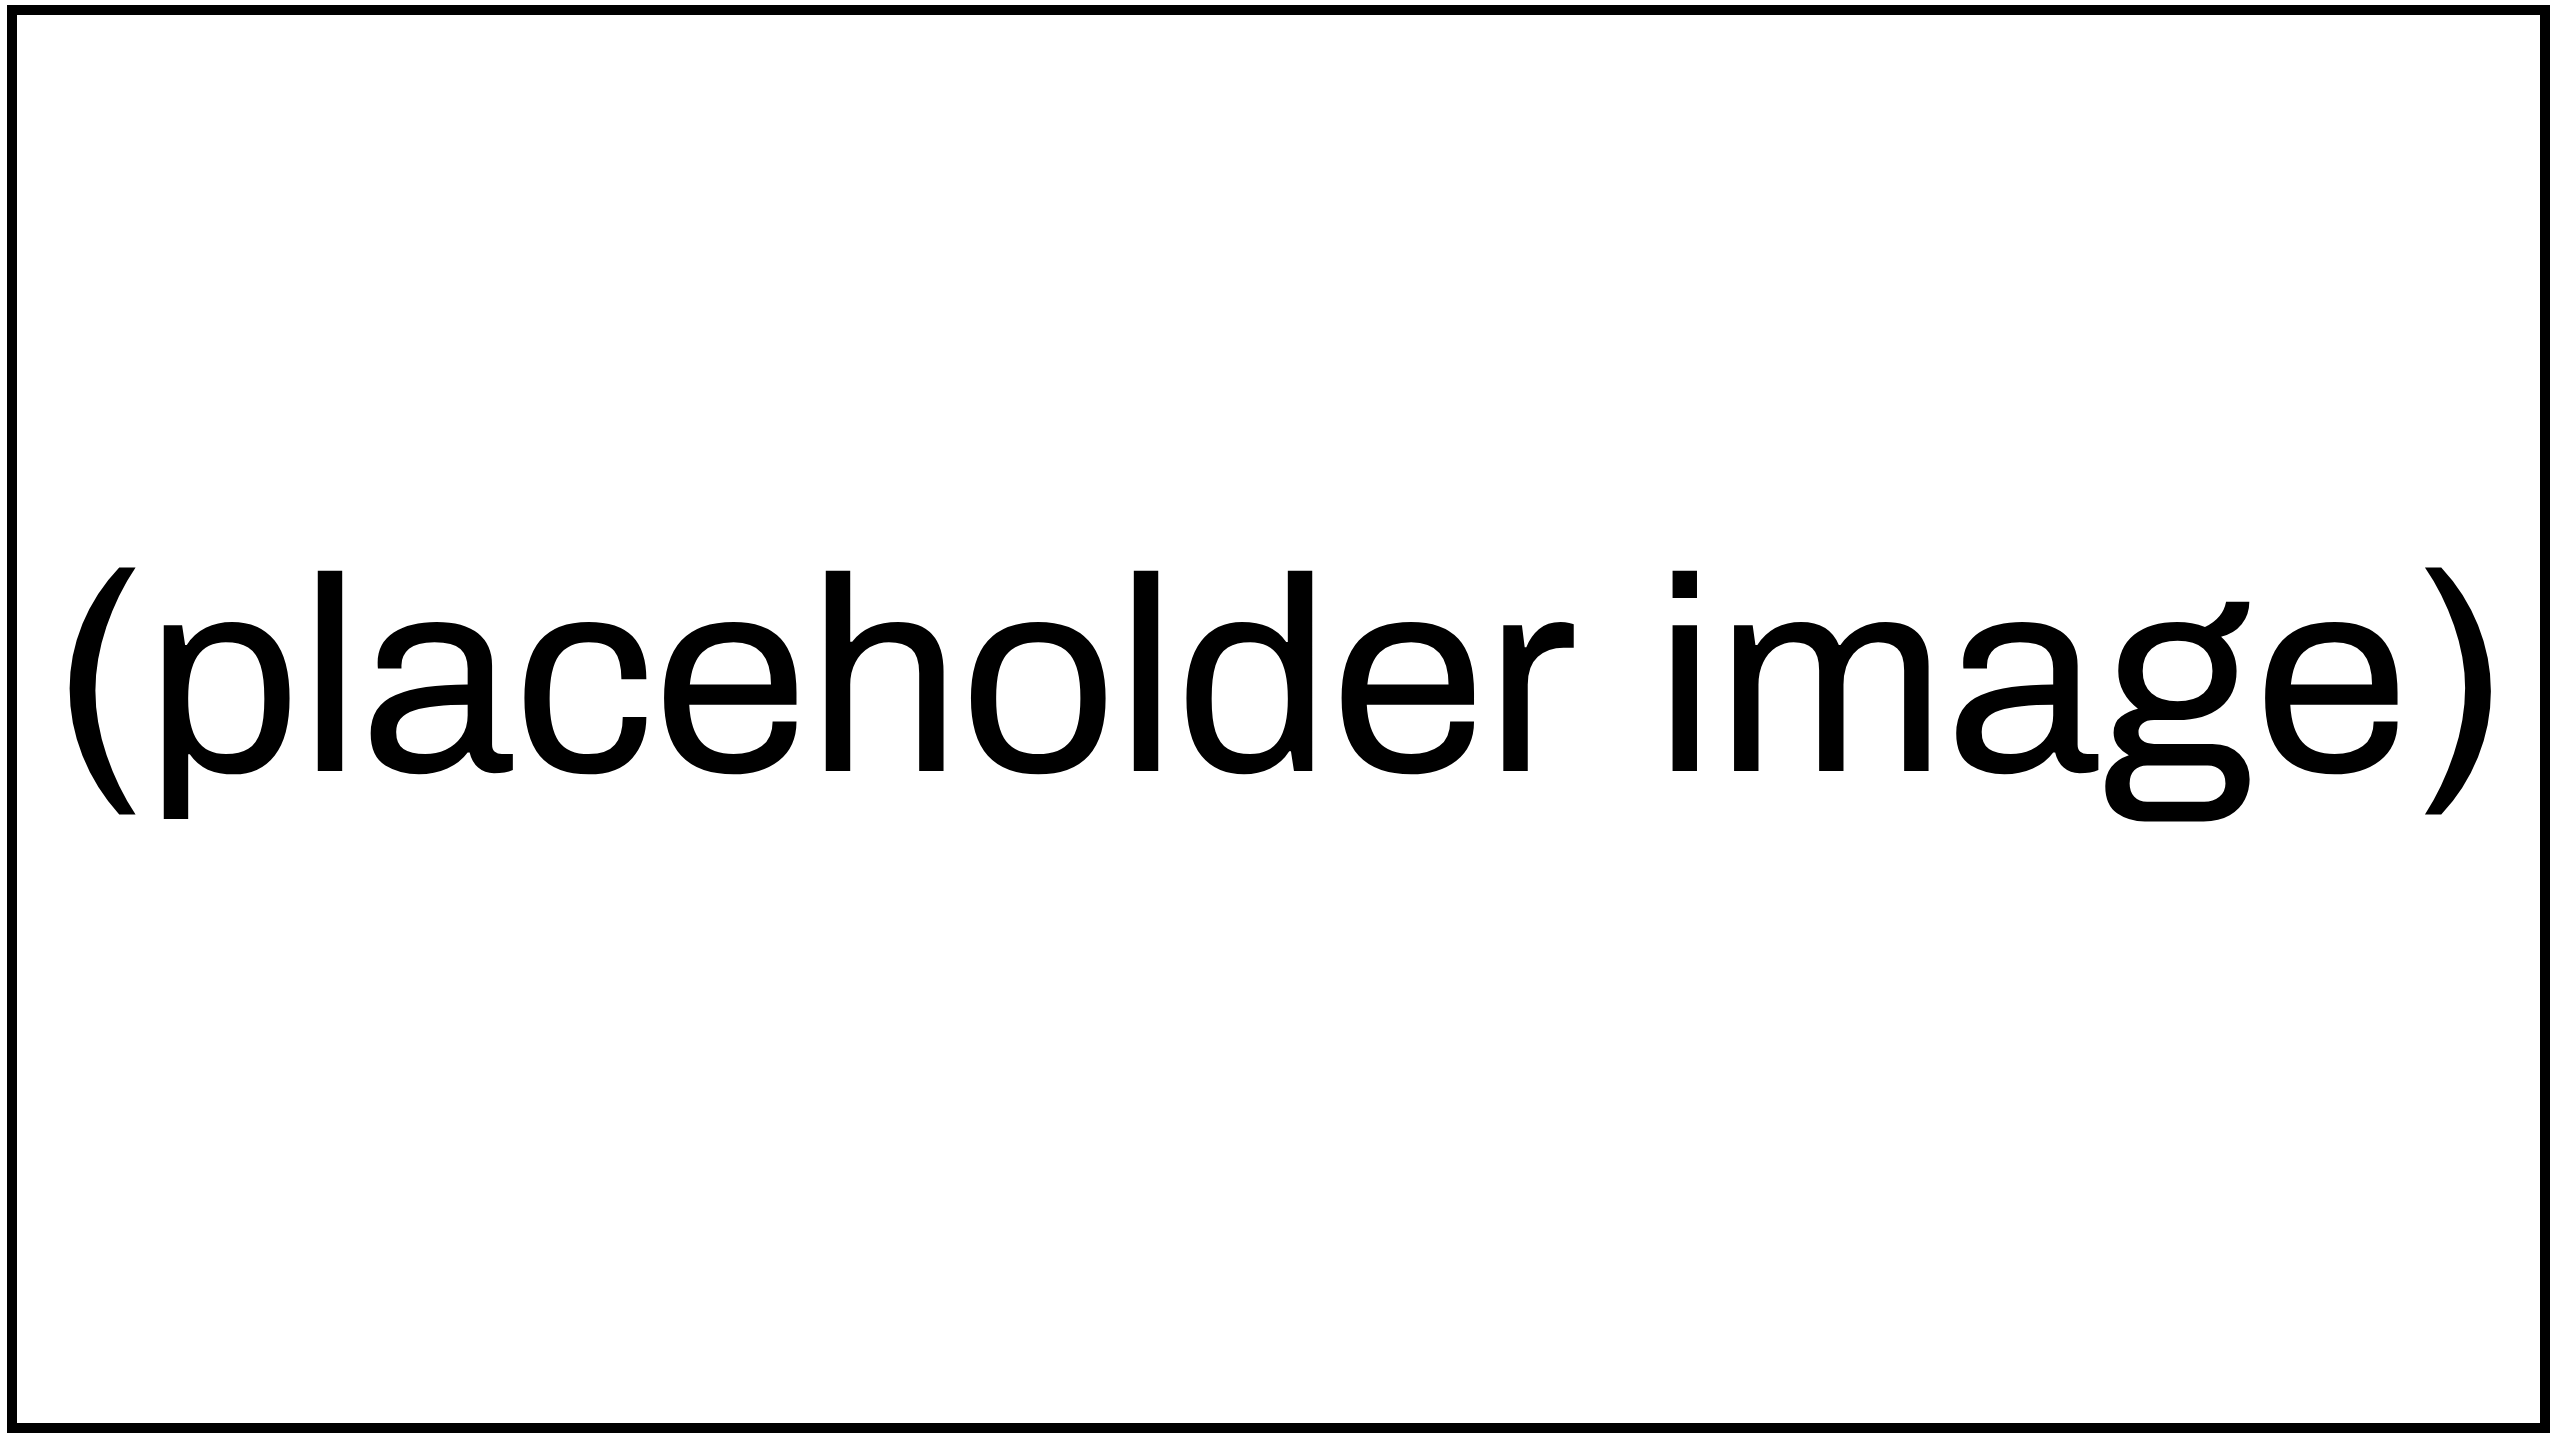
\includegraphics[width=0.8\textwidth]{figures/methodology/placeholder_image.png}
    \caption{SMKIT System Architecture Overview}
    \label{fig:system_architecture_overview}
\end{figure}

The diagram above illustrates how these components are structured and interact with one another to create a streamlined system for automating content generation and distribution.
\end{comment}

\subsection{Technological Stack}
\label{subsec:technological_stack}
The SMKIT project employs a variety of technologies and tools to ensure efficient and effective implementation of its components. The system's design relies primarily on \textit{Python}, a versatile programming language, which serves as the backbone for the development of all key modules. Below is a detailed description of the key technologies used in the project:

\begin{itemize}
    \item \textbf{Python}: \textit{Python} was selected as the primary programming language due to its ease of use, extensive library support, and suitability for web scraping, data manipulation, and automation tasks. The SMKIT system is built entirely in Python, utilizing its powerful libraries for a variety of tasks, from data extraction to content generation and posting.
    
    \item \textbf{argparse}: For managing command-line interfaces, the project uses the \textit{argparse} module. This module simplifies the process of handling command-line arguments, enabling users to interact with the system via terminal commands for various operations permitted by SMKIT.

    \item \textbf{BeautifulSoup}: \textit{BeautifulSoup} is used for web scraping tasks, specifically for extracting metadata and content from external websites. It simplifies the process of navigating HTML structures and retrieving relevant data from web pages.

    \item \textbf{matplotlib}: For visualizing data, the \textit{matplotlib} library is employed to generate plots and diagrams. This is particularly useful for representing the anger and conflict-based metrics derived from data.
    
    \item \textbf{facebook-sdk} and \textbf{tweepy}: These libraries are used to integrate the system with social media platforms like Facebook and Twitter, respectively. The \textit{facebook-sdk} allows for smooth interaction with the Facebook API for posting content, while \textit{tweepy} is used to manage content on Twitter. These libraries are integral in automating the process of sharing content on social media platforms, as discussed in Chapter 2.

\end{itemize}

Each of these technologies plays a vital role in the implementation of SMKIT, ensuring that the system operates efficiently, allowing for smooth data processing, content creation, and automation. The choice of Python, along with its extensive ecosystem of libraries, provides the flexibility needed to handle the diverse tasks within the system.

\subsection{Module Development for Negapedia Integration}
\label{subsec:module_development_negapedia}
Explain the development of the specific module created to integrate data from Negapedia, highlighting any key challenges or innovations.

\section{Data Collection and Preparation}
\label{sec:data_collection_preparation}
This section describes how data is gathered, processed, and prepared for use in the SMKIT system.

\subsection{Web Scraping Tools and Techniques}
\label{subsec:web_scraping_tools_techniques}
Discuss the web scraping tools and techniques employed, such as BeautifulSoup or Scrapy, and how they were used to extract data from web pages.

\subsection{Data Cleaning}
\label{subsec:data_cleaning}
Explain the methods used to clean and process the raw data, including handling missing values, removing duplicates, and correcting errors.

\subsection{Data Transformation}
\label{subsec:data_transformation}
Describe the process of transforming raw data into a usable format for the system, such as converting text into structured data or normalizing values.

\section{Implementation}
\label{sec:implementation}
This section details the implementation of SMKIT, including the development of key modules and the integration of components.

\subsection{Module for Content Automation}
\label{subsec:module_for_content_automation}
Explain how the module for content automation was developed, including the algorithms or logic used to generate posts or content for social media platforms.

\subsection{Integration with Negapedia}
\label{subsec:integration_with_negapedia}
Describe how Negapedia’s data is integrated into the SMKIT system, focusing on the specific integration methods or APIs used.

\subsection{Social Media Platform Integration}
\label{subsec:social_media_integration}
Discuss the methods used to integrate SMKIT with social media platforms (e.g., Twitter, Facebook, Instagram) for automatic content sharing.

\section{Challenges and Limitations}
\label{sec:challenges_limitations}
This section discusses any technical, logistical, or methodological challenges encountered during the project, as well as the limitations of SMKIT.

\subsection{Technical Challenges}
\label{subsec:technical_challenges}
Describe the technical difficulties faced during development, such as integrating with social media APIs or dealing with large-scale data extraction.

\subsection{Limitations of SMKIT}
\label{subsec:limitations_of_smkit}
Explain the limitations of the SMKIT system, including any features or capabilities that are yet to be implemented or limitations in performance.

\section{Conclusion}
\label{sec:methodology_conclusion}
Summarize the key points of the methodology, reflect on the approach taken, and provide a brief transition to the next chapter, which will focus on the **Implementation** or **Results** of SMKIT.
